
\documentclass[%
    25pt, a1paper, portrait,%
    blockverticalspace=15pt,%
    colspace=15pt,%
    margin=0pt,%
    innermargin=20pt,%
]{tikzposter}

%%%%%%%%%%%%%%%%%%%%%%%%%%%%%%%%%%%%%%%%%%%%
% PACKAGES
%%%%%%%%%%%%%%%%%%%%%%%%%%%%%%%%%%%%%%%%%%%%

\usepackage[english]{babel}
\usepackage{amsmath, amsthm, amssymb, latexsym}
\usepackage[utf8]{inputenc}
\usepackage{etoolbox}
\usepackage{xparse}
\usepackage{subcaption}
\usepackage{blindtext}
\usepackage{geometry}
\usepackage{calculator}
\usepackage[thicklines]{cancel}
\usepackage{tikz}
\usetikzlibrary{positioning}

\input{src/cmds/commons}
\input{src/cmds/commands}

%%%%%%%%%%%%%%%%%%%%%%%%%%%%%%%%%%%%%%%%%%%%
% TITLE
%%%%%%%%%%%%%%%%%%%%%%%%%%%%%%%%%%%%%%%%%%%%

\title{Path Planning with CPD Heuristics}
\author{Massimo Bono$^1$, Alfonso E. Gerevini$^1$, Daniel D. Harabor$^2$, Peter J. Stuckey$^2$}
\date{\today}
\institute{%
    $^1$\setFontSize{42}{Dipartimento Di Ingegneria dell'Informazione, Università degli Studi di Brescia, Brescia, Italy}%
    \\%
    $^2$\setFontSize{42}{Faculty of Information Technology, Monash University, Melbourne, Australia}%
}

%%%%%%%%%%%%%%%%%%%%%%%%%%%%%%%%%%%%%%%%%%
% STYLE
%%%%%%%%%%%%%%%%%%%%%%%%%%%%%%%%%%%%%%%%%%

\usetheme{Autumn}
\usecolorstyle[colorPalette=BrownBlueOrange]{Germany}

%%%%%%%%%%%%%%%%%%%%%%%%%%%%%%%%%%%%%%%%%%
% configuration of tikzposter
%%%%%%%%%%%%%%%%%%%%%%%%%%%%%%%%%%%%%%%%%%

%remove logo https://tex.stackexchange.com/a/263278/145331
\tikzposterlatexaffectionproofoff

%%%%%%%%%%%%%%%%%%%%%%%%%%%%%%%%%%%%%%%%%%
% TIKZ CONFIGURATION
%%%%%%%%%%%%%%%%%%%%%%%%%%%%%%%%%%%%%%%%%%

\tikzset{Vertex/.style={%
    shape=circle,%
    draw=blue!30,%
    fill=blue!15,%
    minimum size=10pt,%
    line width=4pt,%
    radius=1cm,%
    inner sep=3pt,%
    node distance=3.5cm,%
}}
\tikzset{StartVertex/.style={%
    shape=circle,%
    draw=blue!50,%
    fill=blue!30,%
    minimum size=10pt,%
    line width=7pt,%
    radius=1cm,%
    inner sep=3pt,%
    node distance=3.5cm,%
}}
\tikzset{TargetVertex/.style={%
    shape=circle,%
    draw=blue!50,%
    fill=blue!30,%
    minimum size=10pt,%
    line width=7pt,%
    radius=1cm,%
    inner sep=3pt,%
    node distance=3.5cm,%
}}
\tikzset{NormalEdge/.style={%
    -.,
    line width=2pt,%
}}
\tikzset{EdgePath/.style={%
    ->,%
    line width=5pt,%
}}
\NewDocumentCommand{\edgeLabel}{s m}{%
    \IfBooleanTF{#1}{%
        \Large{\textbf{\color{red}#2}}%
    }{%
        \Large{\textbf{#2}}%
    }%
}

%%%%%%%%%%%%%%%%%%%%%%%%%%%%%%%%%%%%%%%%%%%%
% DOCUMENT
%%%%%%%%%%%%%%%%%%%%%%%%%%%%%%%%%%%%%%%%%%%%

\begin{document}

    \maketitle
    
    \block{Abstract}{%
        Compressed Path Databases (CPDs) are a leading technique for optimal pathfinding in graphs with static edge costs. In this work we investigate CPDs as admissible heuristic functions and we apply them in two distinct settings: problems where the graph is subject to dynamically changing costs, and anytime settings where deliberation time is limited. Conventional heuristics derive cost-to- go estimates by reasoning about a tentative and usually infeasible path, from the current node to the target. CPD-based heuristics derive cost-to-go estimates by computing a concrete and usually feasible path. We exploit such paths to bound the optimal solution, not just from below but also from above. We demonstrate the benefit of this approach in a range of experiments on standard gridmaps and in comparison to Landmarks, a popular alternative also developed for searching in explicit state-spaces.
    }

    \block{Problem}{%
        \begin{minipage}{0.31\textwidth}%
            \centering%
            \textbf{Original map}%
            \medskip\medskip\medskip

            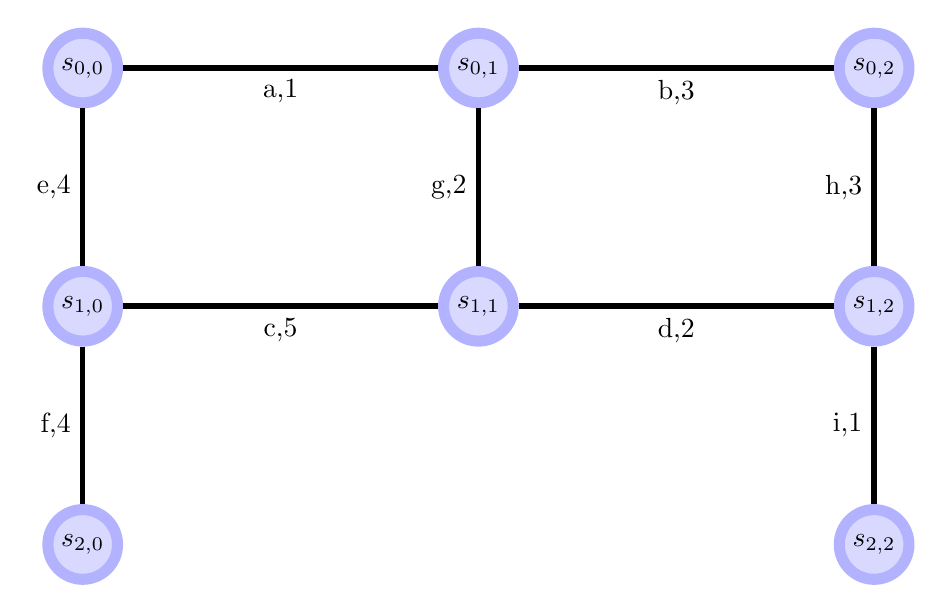
\begin{tikzpicture}
    \node[Vertex] (v00) at (0,0) {$s_{0,0}$};
    \node[Vertex, right=4.0cm of v00] (v01) {$s_{0,1}$};
    \node[Vertex, right=4.0cm of v01] (v02) {$s_{0,2}$};
    \node[Vertex, below=2.0cm of v00] (v10) {$s_{1,0}$};
    \node[Vertex, right=4.0cm of v10] (v11) {$s_{1,1}$};
    \node[Vertex, right=4.0cm of v11] (v12) {$s_{1,2}$};
    \node[Vertex, below=2.0cm of v10] (v20) {$s_{2,0}$};
    \node[Vertex, below=2.0cm of v12] (v22) {$s_{2,2}$};

    \path (v00) edge[NormalEdge] node[below]{\edgeLabel{a,1}} (v01);
    \path (v01) edge[NormalEdge] node[below]{\edgeLabel{b,3}} (v02);
    \path (v10) edge[NormalEdge] node[below]{\edgeLabel{c,5}} (v11);
    \path (v11) edge[NormalEdge] node[below]{\edgeLabel{d,2}} (v12);
    \path (v00) edge[NormalEdge] node[left]{\edgeLabel{e,4}} (v10);
    \path (v10) edge[NormalEdge] node[left]{\edgeLabel{f,4}} (v20);
    \path (v01) edge[NormalEdge] node[left]{\edgeLabel{g,2}} (v11);
    \path (v02) edge[NormalEdge] node[left]{\edgeLabel{h,3}} (v12);
    \path (v12) edge[NormalEdge] node[left]{\edgeLabel{i,1}} (v22);
\end{tikzpicture}
        \end{minipage}%
        \begin{minipage}{0.31\textwidth}
            \centering
            \textbf{Solution of query $\mathbf{q = (s_{0,0}, s_{2,2})}$}
            \medskip\medskip\medskip
            
            \input{src/tikzs/originalgraphquery.tikz}
        \end{minipage}%
        \begin{minipage}{0.31\textwidth}
            \centering
            \textbf{Problem: compute soltuion of $\mathbf{q}$ over map with \textit{perturbations}?}
            \medskip\medskip\medskip
            
            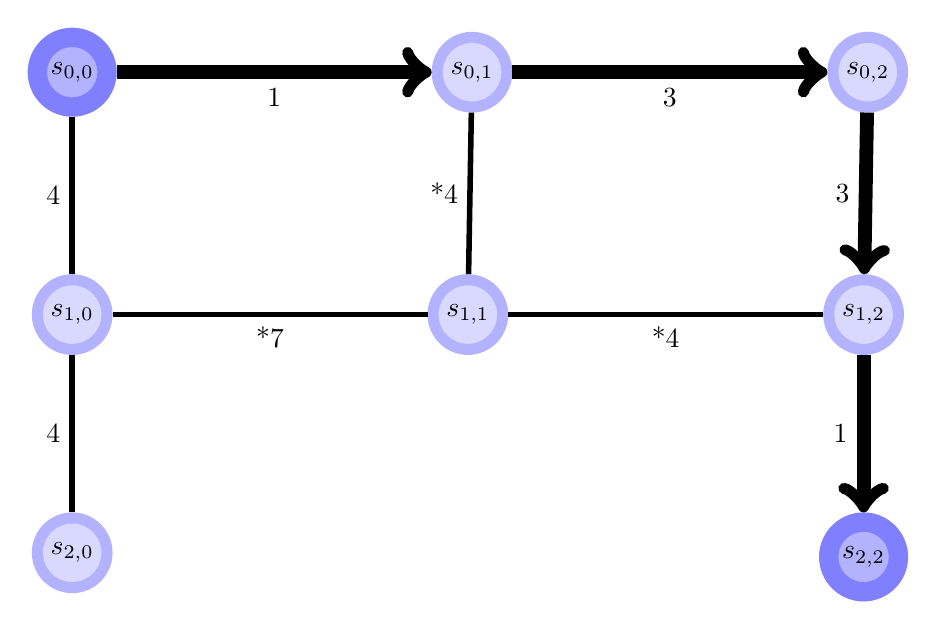
\begin{tikzpicture}
    \node[StartVertex] (v00) at (0,0) {$s_{0,0}$};
    \node[Vertex, right=4.0cm of v00] (v01) {$s_{0,1}$};
    \node[Vertex, right=4.0cm of v01] (v02) {$s_{0,2}$};
    \node[Vertex, below=2.0cm of v00] (v10) {$s_{1,0}$};
    \node[Vertex, right=4.0cm of v10] (v11) {$s_{1,1}$};
    \node[Vertex, right=4.0cm of v11] (v12) {$s_{1,2}$};
    \node[Vertex, below=2.0cm of v10] (v20) {$s_{2,0}$};
    \node[TargetVertex, below=2.0cm of v12] (v22) {$s_{2,2}$};

    \path (v00) edge[EdgePath] node[below]{\edgeLabel{1}} (v01);
    \path (v01) edge[EdgePath] node[below]{\edgeLabel{3}} (v02);
    \path (v10) edge[NormalEdge] node[below]{\edgeLabel*{7}} (v11);
    \path (v11) edge[NormalEdge] node[below]{\edgeLabel*{4}} (v12);
    \path (v00) edge[NormalEdge] node[left]{\edgeLabel{4}} (v10);
    \path (v10) edge[NormalEdge] node[left]{\edgeLabel{4}} (v20);
    \path (v01) edge[NormalEdge] node[left]{\edgeLabel*{4}} (v11);
    \path (v02) edge[EdgePath] node[left]{\edgeLabel{3}} (v12);
    \path (v12) edge[EdgePath] node[left]{\edgeLabel{1}} (v22);
\end{tikzpicture}
        \end{minipage}%
    }

    \block{\CPDSearch{} $\Rightarrow$ Exploit \CPD{} in \A{} variant}{%
        \begin{minipage}{0.31\textwidth}
            \centering
            \textbf{Admissible heuristic}
            \medskip\medskip\medskip

            \input{src/tikzs/admissibleheuristic.tikz}            
        \end{minipage}%
        \begin{minipage}{0.31\textwidth}
            \centering
            \textbf{Early Termination}
            \medskip\medskip\medskip

            \input{src/tikzs/admissibleheuristic.tikz}            
        \end{minipage}%
        \begin{minipage}{0.31\textwidth}
            \centering
            \textbf{Obtain solution bounds}
            \medskip\medskip\medskip

            \input{src/tikzs/admissibleheuristic.tikz}            
        \end{minipage}

    }

    \begin{columns}
        \column{0.64}{%
            \block{Optimal scenario}{%
                \begin{minipage}{0.5\linewidth}
                    \centering
                    \includegraphics[width=1.0\linewidth]{src/images/maze512-1-4}
                \end{minipage}\hfill%
                \begin{minipage}{0.5\linewidth}
                    \centering
                    \includegraphics[width=1.0\linewidth]{src/images/hrt201n}
                \end{minipage}
            }
        }%
        \column{0.36}{%
            \block{Anytime scenario}{%
                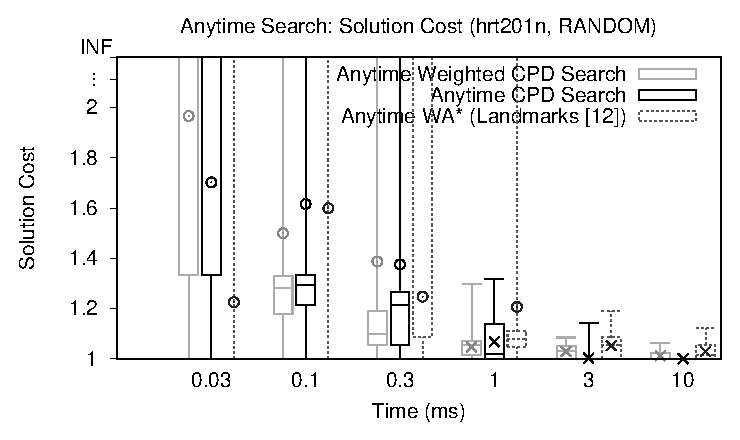
\includegraphics[width=1.0\linewidth]{src/images/anytime}
                %add space to fill everything
                \medskip
                \phantom{x}
            }
        }
    \end{columns}
    
\end{document}